%----------------------------------------------------------------------------------------
%	CONFIGURATIONS
%----------------------------------------------------------------------------------------

\documentclass[12pt,a4paper,oneside]{article}

\usepackage[utf8]{inputenc}
\usepackage[colorlinks=true, citecolor=blue, linkcolor=black]{hyperref}
\usepackage{graphicx}
% \usepackage{natbiba}
\usepackage{amsmath}
\usepackage{caption}
\usepackage{subcaption}
\graphicspath{ {images/} }
\usepackage[a4paper,left=2cm,right=2cm,top=2.5cm,bottom=2.5cm]{geometry}
\setcounter{section}{-1}

%----------------------------------------------------------------------------------------
%	INFORMATION
%----------------------------------------------------------------------------------------

\title{Tópicos Avançados em Algoritmos (TAA) - Practical Assignment 1}

\author{João Rebelo Pires\footnote{João Rebelo Pires - 201200384} and José Miguel Oliveira\footnote{José Miguel Oliveira - 201304192}}

\date{DCC - FCUP, April 2017}

\begin{document}

\maketitle

%----------------------------------------------------------------------------------------
%	SECTION 0
%----------------------------------------------------------------------------------------

\section{How To}\label{sec:for_dummies}

In this section, we simply want to explain how to compile and execute our implementation.

\subsection{Input Description}\label{subsec:input_descrip}

The first line of input contains a single integer, an option. If this option is $0$, we are looking for the horizontal partition. Alternatively, the option may be $1$, indicating that we are looking for the grid partition.

The second line of input is an integer, $n\_vertices$, describing the number of vertices the orthogonal polygon has. Then $n\_vertices$ lines follow, the coordinates of the vertices of the polygon, given in counterclockwise order. The coordinates are integer.

The next line of input is an integer, $n\_holes$, describing the number of holes the polygon has. The following lines describe each hole, ina  similar way as the polygon is described.

\subsection{Output Description}\label{subsec:output_descrip}

The output is well represented. It consists on three groups of information.

\begin{enumerate}
	\item The description of each vertex of the DCEL;
	\item The description of each face of the DCEL;
	\item The description of each half edge of the DCEL.
\end{enumerate}

The information each element of the DCEL provides is discussed in Section \ref{sec:dcel}.

\subsection{Compilation}\label{subsec:compile}

The following command line compiles the code:

\textit{In MacOS X:}

\texttt{clang++ -Wall main.cpp code/dcelutil.cpp}\\

\textit{In Linux:}

\texttt{c++ -Wall main.cpp code/dcelutil.cpp}

\subsection{Execution}

The compiler generates an executable named \textbf{a.out}. To execute it, simply execute the following command line:

\texttt{./a.out}.\\

If you have an input file \textbf{test.in}, you should execute the following command line instead:

\texttt{./a.out < test.in}.

%----------------------------------------------------------------------------------------
%	SECTION 1
%----------------------------------------------------------------------------------------
\section{Introduction}\label{sec:intro}
For this assignment we had the task of partitioning any orthogonal polygon with or without holes, then compute the visibility and finally study experimentally the minimum guard problem. 

Our algorithm gives the complete horizontal partition. As for the grid partition, we did not manage to complete it, but what is left to implement of our strategy is discussed in Section \ref{sec:grid}.

%----------------------------------------------------------------------------------------
%	SECTION 2
%----------------------------------------------------------------------------------------
\section{The Doubly Connected Edge List Structure}\label{sec:dcel}
To represent the polygon with and without the partitions we use a Doubly Connected Edge List (DCEL), as it provides important operations over the representation to be time efficient, as it is discussed by Marc van Kreveld\footnote{\textit{Computational Geometry -
Lecture 2b: Subdivision representation and map overlay}, \url{http://www.cs.uu.nl/docs/vakken/ga/slides2b.pdf}}.\\
This structure allows us to easily build and traverse the polygon, as it is built using the half edges of the polygon and each half edge has the following attributes:

\begin{enumerate}  
\item \textbf{Next}: The half edge that comes after the one we are analysing;
\item \textbf{Incident}: The face in which that half edge is contained;
\item \textbf{Twin}: The reverse half edge to the one we are analysing, used to navigate through the polygon in reverse;
\item \textbf{Prev}: The half edge that comes before the one we are analysing;
\item \textbf{Origin}: The vertex from which this half edge originates.
\end{enumerate}

\begin{figure}[h!]
  \centering 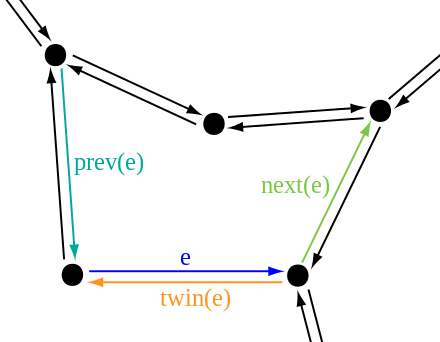
\includegraphics[scale=0.5]{dcel.png}
  \caption{Visual representation of a DCEL.}
  \label{fig:Dcel}
\end{figure}

% https://upload.wikimedia.org/wikipedia/commons/thumb/0/07/Dcel-halfedge-connectivity.svg/440px-Dcel-halfedge-connectivity.svg.png

Using these attributes we can easily print out the polygon and its partitions using the next attributes to navigate through each different face.

\pagebreak

%----------------------------------------------------------------------------------------
%	SECTION 3
%----------------------------------------------------------------------------------------
\section{Horizontal Partition}\label{sec:hor}
In order to obtain the horizontal partition, our algorithm uses a sweep line premise.\\ 
In order to obtain this, we first determine a list of events, as described by Prof. Ana Paula Tomás\footnote{\url{http://www.dcc.fc.up.pt/Pubs/TR04/dcc-2004-03.ps.gz}}, which are horizontal half-edges with its incident face being a face inside the polygon. \\
Let us look at an example:

\begin{figure}[h!]
  \centering 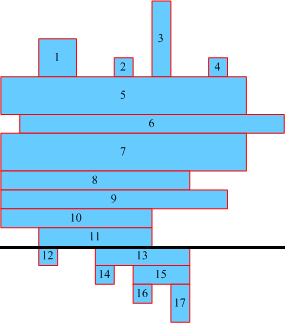
\includegraphics[scale=0.5]{horPartition.png}
  \caption{Horizontal Partition}
  \label{fig:hor}
\end{figure}

% http://www.yzuda.org/download/_CornerStitchingStrips/complex-02.png

The figure above, shows us how the horizontal partition of an orthogonal polygon.

The black horizontal line is the sweep line, that goes from event to event looking for possible edge extensions. Each event is a horizontal half-edge, as described before.

We can see the different types of intersections that occur, which we mentioned previously. The intersection between two inside vertexes, as we can see at the bottom of rectangle 6, and the intersection between an inside vertex and the vertical polygon edge that can be seen at the top of the rectangle numbered 9.

\subsection{Description of Data Structures Used and Others}\label{subsec:data}

First of all, let us notice that since this is a geometric problem, a lot of geometric primitives are useful. The file \texttt{geoutil.h} includes a series of such primitives that we considered of relevance. The file \texttt{dcelutil.h} also includes the functions \texttt{rotateCCW90} and \texttt{rotateCW90}, which are useful in Section \ref{sec:grid}, that simply rotate a given point $90^{\circ}$ in counterclockwise and clockwise directions, respectively.

The files \texttt{dcelutil.h} and \texttt{dcelutil.cpp} put together the implementation of the major functions of our implementation. Let us take a couple for illustration:

\begin{itemize}
	\item \texttt{init\_poly}, which given the points of a polygon in counterclockwise direction constructs the DCEL that represents such polygon;
	\item \texttt{print\_dcel}, that prints the contents of the DCEL;
	\item \texttt{sweep\_line}, that performs an $n$ $log\left( n \right)$ horizontal sweep through the polygon;
	\item \texttt{init\_hole}, which adds a hole to the DCEL representation given the points in clockwise direction.
\end{itemize}

These functions use within themselves functions like \texttt{splitHalfEdgeL}, that given an event, if by extending it we intersect a side of the polygon and this segment lyes completely inside the polygon, divides that segment in two, creating also two different faces induced by this division. It is observable that this division does not always induce two different faces (because of the holes), but since given a half-edge its next component lyes on the same face as such half-edge, \texttt{create\_face\_from} assures that they are given the same face.

This function, \texttt{splitHalfEdgeL}, can be used in two different situations:

\begin{enumerate}
	\item If the event is from right to left, the edge of the polygon is on its left, and on the left of such event there is a piece that goes \textit{upwards} in our polygon;
	\item If the event is from left to right, the edge of the polygon is on its right, and on the right of such event there is a piece that goes \textit{downwards} in our polygon.
\end{enumerate}

\texttt{splitHalfEdgeR} can be used for the other two cases that we can get.

\subsection{\texttt{map} Data Structure in \texttt{C++} and the State of the Sweep Line}

For representing the state of the sweep line we used a \texttt{map} in \texttt{C++}, since they are implemented as red-black trees, which provide searching, removing and inserting operations in $log(n)$, giving a complexity for the sweep line algorithm of $n$ $log(n)$, where $n$ is the number of edges.

\texttt{set} is another data structure in \texttt{C++} implemented using red-black trees.

\subsection{Bulletproofness of our Implementation}\label{subsec:bullet}

One question that rises is why is the grid partition not complete, as well as the second and third questions.

In this subsection we discuss why it took us so long to build the horizontal partition.

The first observation is that, contrary to what we had expected, it is equivalent for the purpose of constructing partitions for a polygon to have holes or not. Our algorithm does not partition the inside face of a hole, since the half-edges that lye inside it are never added neither to the events nor to the state of the sweep line.

So where is the problem? The problem is with the fact that the polygon, as well as the holes, can have collinear edges. This makes the task of building a partition harder, since we may need to add edges related to an unprocessed event in an event before. In order to make sure that the partition is well constructed, a lot of different cases needed to be considered, and in order to accomplish a bulletproof algorithm, we spent a lot of time thinking about every single possible case that might arise. Even so, we spent way too long fixing problems and bugs in our implementation that would not pass our \textit{bulletproofness test} cases. Some are described in section \ref{sec:input_final}.

%----------------------------------------------------------------------------------------
%	SECTION 4
%----------------------------------------------------------------------------------------
\section{Grid Partition}\label{sec:grid}

In order to get the grid partition, we tried to think a bit out of the box, giving an idea that used most of the code we already had. Our implementation idea is as follows:

\begin{itemize}
	\item We begin by rotating the polygon $90^{\circ}$ in CCW (we can revert this by rotating it $90^{\circ}$ in CW) and is illustrated in Figure \ref{fig:rot};
	\item We semi-construct the partition induced by a horizontal sweep on such rotated polygon;
	\item This semi-construction is achieved simply by storing the points of intersection of the extensions of the events with the sides of the polygon, as well as the direction of the inside half-edge, given its endpoints' vertexes' indexes (which are preserved after rotations);
	\item In the DCEL representing the horizontal partition, add these points, that we call \textbf{interest points}, to the representation, dividing the horizontal edges of the polygon accordingly;
	\item Since the grid partition produces faces that are rectangles, and we already have all interest points on the sides of the polygon (and on the sides of the holes, if any), we can now search for the rectangles in a way that if a face is not a rectangle, make it a rectangle. If the four endpoints of such polygon already exist, simply connect the two that are not connected, and create two new faces for each of the two faces induced by this connection. If one of the endpoints does not exist, we know that we are handling an extension of a horizontal event that needs to be divided in two. This idea is better explained with an example in Section \ref{subsec:gridex}.
\end{itemize}

\begin{figure}[h!]
  \centering 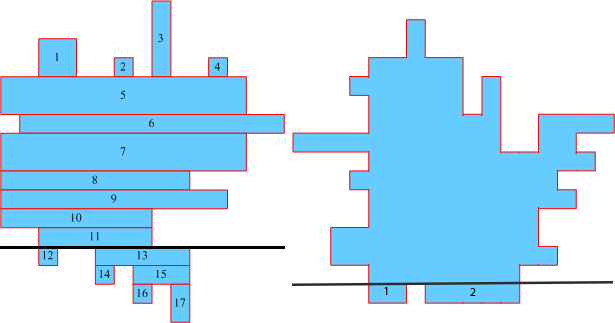
\includegraphics[scale=0.5]{rotatedPoly.png}
  \caption{Polygon Rotation Example.}
  \label{fig:rot}
\end{figure}

An example of a grid partition is given in Figure \ref{fig:grid}.

\begin{figure}[h!]
  \centering 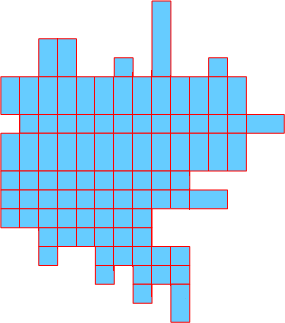
\includegraphics[scale=0.5]{gridPartition.png}
  \caption{Grid Partition Representation.}
  \label{fig:grid}
\end{figure}

The first four points of our idea for the grid partition are implemented and working. If we give the option to construct the grid partition, our algorithm already prints the DCEL after adding the interest points.

Unfortunately, we were not able to complete the last one.

\subsection{Our Idea for the Grid Partition - An Example}\label{subsec:gridex}

Consider the example in Figure \ref{fig:idea}.

\begin{figure}[h!]
  \centering 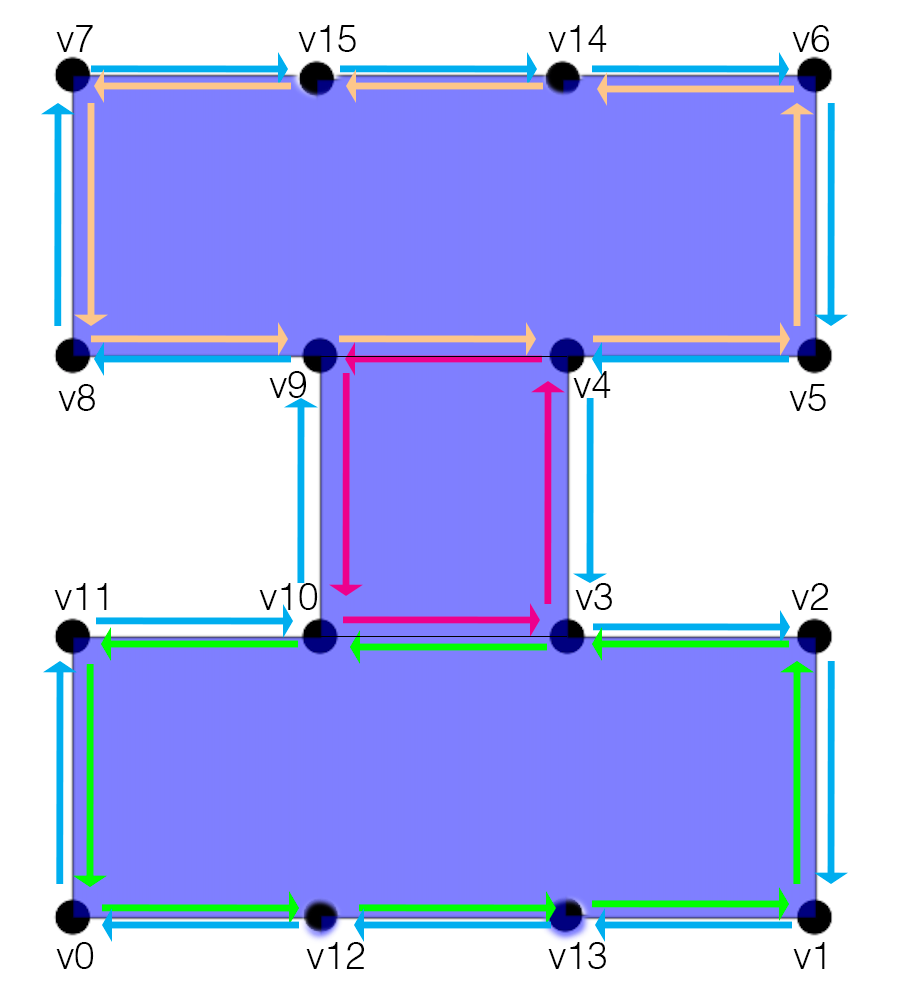
\includegraphics[scale=0.2]{second.png}
  \caption{Polygon with a horizontal partition.}
  \label{fig:idea}
\end{figure}

In this example, we do not need to divide any extensions of events.

First of all, we need to get the horizontal half-edges that are candidates for searching for rectangles. We can do this in linear time on the number of rectangles generated by the grid partition, using the map of half-edges (that maps vertex indexes $v_{i}, v_{j}$ into half-edges with direction $\overrightarrow{v_{i} v_{j}}$), alongside with the faces (ordered first by $y$ and then by $x$; we can also use a map for this).

Then, we proceed as we explain with an example so it is easier to understand our idea. Let us take half-edge $\overrightarrow{v_{0}  v_{12}}$, for instance. If we search for two previous half-edges prior to that, we get to $\overrightarrow{v_{10} v_{11}}$. Since the origin of this half-edge has already $x$-coordinate same as $v_{0}$, we do not need to divide half-edge $\overrightarrow{v_{10} v_{11}}$. On the other hand, since the half-edge previous to $\overrightarrow{v_{10} v_{11}}$ is not a half-edge with origin $v_{12}$, we need to connect $v_{12}$ to $v_{10}$, and $v_{10}$ to $v_{12}$.

We continue to do this until we have no more faces to visit, obtaining then the grid partition as we desired.

%----------------------------------------------------------------------------------------
%	SECTION 5
%-----------------------

\section{Input Tests and Final Remarks}\label{sec:input_final}

These were some tests we used to test the \textit{bulletproofness} of our algorithm:
\begin{itemize}
	\item Test 1:

1

20

0 0

9 0

9 1

8 1

8 3

7 3

7 2

6 2

6 3

5 3

5 1

4 1

4 3

3 3

3 2

2 2

2 3

1 3

1 1

0 1

0

	\item Test 2 (with a hole and in Figure \ref{fig:hole}):

0

12

0 0

5 0

5 4

4 4

4 3

3 3

3 4

2 4

2 3

1 3

1 4

0 4

1

4

2 1

2 2

3 2

3 1

	\item Test 3:

0

16

0 5

2 5

2 3

4 3

4 1

6 1

6 0

7 0

7 2

5 2

5 4

3 4

3 6

1 6

1 7

0 7

	\item Test 4 (in Figure \ref{fig:idea}, with its output also visually represented):

1


12

0 0

3 0

3 1

2 1

2 2

3 2

3 3

0 3

0 2

1 2

1 1

0 1

0

\end{itemize}

\begin{figure}[h!]
  \centering 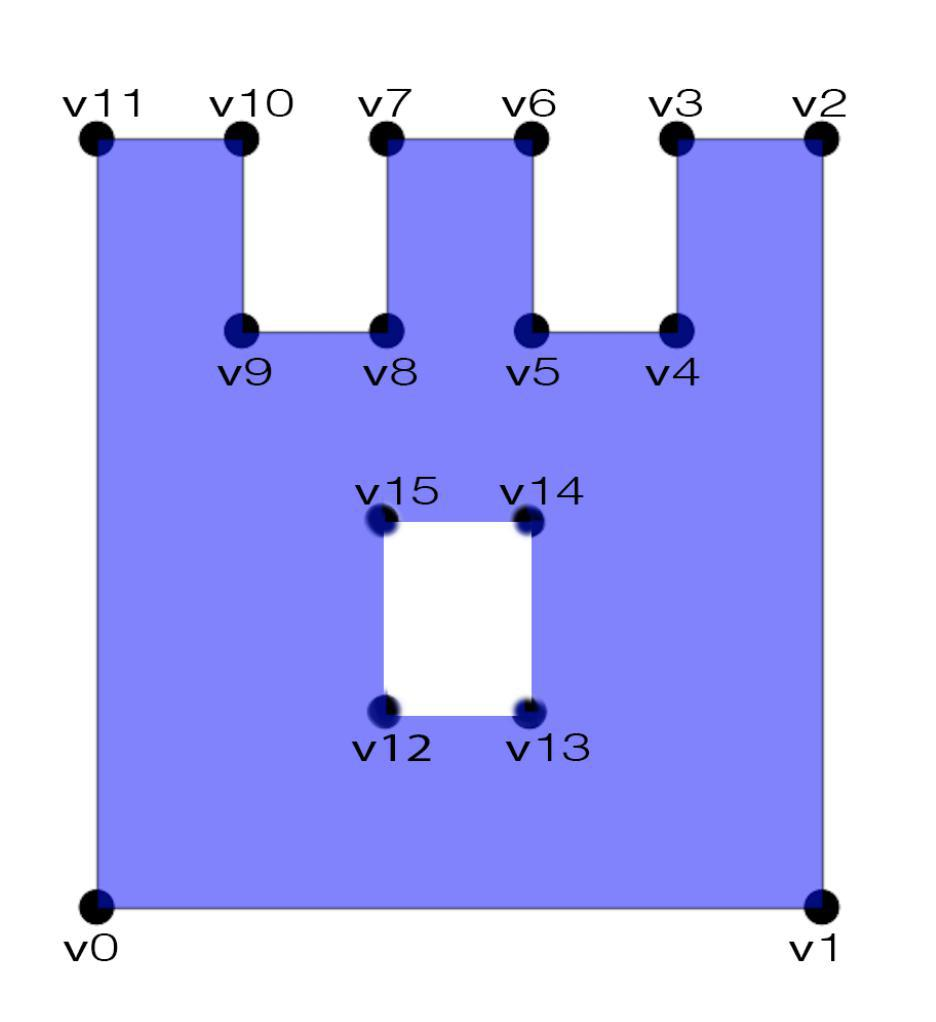
\includegraphics[scale=0.2]{first.jpg}
  \caption{Example of a polygon with one hole.}
  \label{fig:hole}
\end{figure}

This implementation has a complexity $n$ $log(n)$, where $n$ is the number of edges of the polygon, for the sweep based parts. The implementation has output sensitive complexity in some parts, since it depends on the number of rectangles one gets from the grid partition.

\end{document}
